\documentclass[12pt]{article}
\usepackage{lecture}
\usepackage{html}
\usepackage{graphicx}
\usepackage{epstopdf}

\newcommand{\copyrightYears}{2001-2012}

\title{The Hardy-Weinberg Principle and estimating allele frequencies}

\begin{document}

\maketitle

\thispagestyle{first}

\section*{Introduction}

To keep things relatively simple, we'll spend much of our time in this
course talking about variation at a single genetic locus, even though
alleles at many different loci are involved in expression of most
morphological or physiological traits. We'll spend about three weeks
in mid-October studying the genetics of quantitative variation, but
until then you can asssume that I'm talking about variation at a
single locus unless I specifically say otherwise.

\section*{The genetic composition of populations}

When I talk about the genetic composition of a population, I'm
referring to three aspects of variation within that
population:\footnote{At each locus I'm talking about. Remember, I'm
  only talking about one locus at a time, unless I specifically say
  otherwise. We'll see why this matters when we get to two-locus
  genetics in a few weeks.}\index{genetic composition of populations}
\begin{enumerate}

\item The number of alleles at a locus.

\item The frequency of alleles at the locus.

\item The frequency of genotypes at the locus.

\end{enumerate}
It may not be immediately obvious why we need both (2) and
(3) to describe the genetic composition of a population, so let me
illustrate with two hypothetical populations:
\begin{center}
\begin{tabular}{lrrr}
             & $A_1A_1$ & $A_1A_2$ & $A_2A_2$ \\
Population 1 &       50 &        0 &       50 \\
Population 2 &       25 &       50 &       25 \\
\end{tabular}
\end{center}
It's easy to see that the frequency of $A_1$ is 0.5 in both
populations,\footnote{$p_1 = 2(50)/200 = 0.5$, $p_2 = (2(25) + 50)/200
= 0.5$.} but the genotype frequencies are very different. In point of
fact, we don't need both genotype and allele frequencies. We can
always calculate allele frequencies from genotype frequencies, but we
can't do the reverse unless $\dots$

\section*{Derivation of the Hardy-Weinberg principle}

We saw last time using the data from {\it Zoarces viviparus\/} that we
can describe empirically and algebraically how genotype frequencies in
one generation are related to genotype frequencies in the next. Let's
explore that a bit further. To do so we're going to use a technique
that is broadly useful in population genetics, i.e., we're going to
construct a mating table. A mating table consists of three
components:\index{mating table}

\begin{enumerate}

\item A list of all possible genotype pairings.

\item The frequency with which each genotype pairing occurs.

\item The genotypes produced by each pairing.

\end{enumerate}

\begin{center}
\begin{tabular}{rcccc}
\hline\hline
                       &           & \multicolumn{3}{c}{Offsrping genotype} \\
Mating                 & Frequency     & $A_1A_1$ & $A_1A_2$ & $A_2A_2$ \\
\hline
$A_1A_1 \times A_1A_1$ & $x_{11}^2$     &        1 &        0 &        0 \\
              $A_1A_2$ & $x_{11}x_{12}$ &    $\half$ &    $\half$ &        0 \\
              $A_2A_2$ & $x_{11}x_{22}$ &        0 &        1 &        0 \\
$A_1A_2 \times A_1A_1$ & $x_{12}x_{11}$ &    $\half$ &    $\half$ &        0 \\ 
              $A_1A_2$ & $x_{12}^2$     &  $\fourth$ &    $\half$ &  $\fourth$ \\
              $A_2A_2$ & $x_{12}x_{22}$ &        0 &    $\half$ &    $\half$ \\
$A_2A_2 \times A_1A_1$ & $x_{22}x_{11}$ &        0 &        1 &        0 \\
              $A_1A_2$ & $x_{22}x_{12}$ &        0 &    $\half$ &    $\half$ \\   
              $A_2A_2$ & $x_{22}^2$     &        0 &         0 &
                       1 \\
\hline
\end{tabular}
\end{center}
Believe it or not, in constructing this table we've already made three
assumptions about the transmission of genetic variation from one
generation to the next:\index{Hardy-Weinberg assumptions}

\begin{description}

\item[Assumption \#1] Genotype frequencies are the same in males and
  females, e.g., $x_{11}$ is the frequency of the $A_1A_1$ genotype in
  both males and females.\footnote{It would be easy enough to relax
    this assumption, but it makes the algebra more complicated without
    providing any new insight, so we won't bother with relaxing it
    unless someone asks.}

\item[Assumption \#2] Genotypes mate at random {\it with respect to
  their genotype at this particular locus}.

\item[Assumption \#3] Meiosis is fair. More specifically, we assume
  that there is no segregation distortion; no gamete competition; no
  differences in the developmental ability of eggs, or the
  fertilization ability of sperm.\footnote{We are also assuming that
    we're looking at offspring genotypes at the zygote stage, so that
    there hasn't been any opportunity for differential survival.} It
  may come as a surprise to you, but there are alleles at some loci in
  some organisms that subvert the Mendelian rules, e.g., the $t$
  allele in house mice, segregation distorter in {\it Drosophila
    melanogaster}, and spore killer in {\it Neurospora crassa\/}. A
  pair of paper describing the most recent work in {\it Neurospora\/}
  just appeared in July~\cite{Hammond-etal-2012,Saupe-2012}.

\end{description}
Now that we have this table we can use it to calculate the frequency
of each genotype in newly formed zygotes in the
population,\footnote{Not just the offspring from these matings}
provided that we're willing to make three additional assumptions:

\begin{description}

\item[Assumption \#4] There is no input of new genetic material, i.e.,
gametes are produced without mutation, and all offspring are produced
from the union of gametes within this population, i.e., no migration
from outside the population.

\item[Assumption \#5] The population is of infinite size so that the
actual frequency of matings is equal to their expected frequency and
the actual frequency of offspring from each mating is equal to the
Mendelian expectations.

\item[Assumption \#6] All matings produce the same number of
offspring, on average. 

\end{description}
Taking these three assumptions together allows us to conclude that the
frequency of a particular genotype in the pool of newly formed zygotes
is
\[
\sum(\hbox{frequency of mating})(\hbox{frequency of genotype produce
  from mating}) \quad .
\]
So

\begin{eqnarray*}
\hbox{freq.}(A_1A_1\hbox{ in zygotes}) &=&
   x_{11}^2 + \frac{1}{2}x_{11}x_{12} + \frac{1}{2}x_{12}x_{11}
   + \frac{1}{4}x_{12}^2 \\
&=& x_{11}^2 + x_{11}x_{12} + \frac{1}{4}x_{12}^2 \\
&=& (x_{11} + x_{12}/2)^2 \\
&=& p^2 \\
\hbox{freq.}(A_1A_2\hbox{ in zygotes}) &=& 2pq \\
\hbox{freq.}(A_2A_2\hbox{ in zygotes}) &=& q^2 \\
\end{eqnarray*}
Those frequencies probably look pretty familiar to you. They are, of
course, the familiar Hardy-Weinberg proportions. But we're not done
yet. In order to say that these proportions will also be the genotype
proportions of adults in the progeny generation, we have to make two
more assumptions:

\begin{description}

\item[Assumption \#7] Generations do not overlap.

\item[Assumption \#8] There are no differences among genotypes in the
probability of survival.

\end{description}

\section*{The Hardy-Weinberg principle}\index{Hardy-Weinberg principle}

After a single generation in which {\it all\/} eight of the above
assumptions are satisfied

\begin{eqnarray}
\hbox{freq.}(A_1A_1\hbox{ in zygotes}) &=& p^2 \label{eq:hw-p2} \\
\hbox{freq.}(A_1A_2\hbox{ in zygotes}) &=& 2pq \label{eq:hw-2pq} \\
\hbox{freq.}(A_2A_2\hbox{ in zygotes}) &=& q^2 \label{eq:hw-q2} 
\end{eqnarray}

\noindent It's vital to understand the logic here.

\begin{enumerate}

\item If Assumptions \#1--\#8 are true, then equations
  \ref{eq:p2}--\ref{eq:q2} {\bf must} be true.

\item If genotypes are in Hardy-Weinberg proportions, one or more of
  Assumptions \#1--\#8 may still be violated. 

\item If genotypes are {\it not\/} in Hardy-Weinberg proportions, one
  or more of Assumptions \#1--\#8 {\bf must} be false.

\item Assumptions \#1--\#8 are {\it sufficient\/} for Hardy-Weinberg
  to hold, but they are not {\it necessary\/} for Hardy-Weinberg to
  hold. 

\end{enumerate}

Point (3) is why the Hardy-Weinberg principle is so important. There
isn't a population of any organism anywhere in the world that
satisfies all 8 assumptions, even for a single
generation.\footnote{There may be some that come reasonably close, but
  none that fulfill them {\it exactly}. There aren't any populations
  of infinite size, for example.}  But {\it all\/} possible
evolutionary forces within populations cause a violation of at least
one of these assumptions. Departures from Hardy-Weinberg are one way
in which we can detect those forces and estimate their
magnitude.\footnote{Actually, there's a ninth assumption that I didn't
  mention. Everything I said here depends on the assumption that the
  locus we're dealing with is autosomal. We can talk about what
  happens with sex-linked loci, if you want. But again, mostly what we
  get is algebraic complications without a lot of new insight.}

\section*{Estimating allele frequencies}

Before we can determine whether genotypes in a population are in
Hardy-Weinberg proportions, we need to be able to estimate the
frequency of both genotypes and alleles. This is easy when you can
identify all of the alleles within genotypes, but suppose that we're
trying to estimate allele frequencies in the ABO blood group system in
humans. Then we have a situation that looks like this:

\begin{center}
\begin{tabular}{l|r|r|r|r}
\hline\hline
Phenotype      & A      & AB       & B       & O  \\
\hline
Genotype(s)    & aa\ ao & ab       & bb\ bo  & oo \\
No.\ in sample & $N_A$  & $N_{AB}$ & $N_{B}$ & $N_O$ \\
\hline
\end{tabular}
\end{center}
Now we can't directly count the number of $a$, $b$, and $o$
alleles. What do we do? Well, more than 50 years ago, some geneticists
figured out how with a method they called ``gene
counting''~\cite{Ceppellini-etal-1955} and that statisticians later
generalized for a wide variety of purposes and called the EM
algorithm~\cite{Dempster-etal-1977}. It uses a trick you'll see
repeatedly through this course. When we don't know something we want
to know, we pretend that we know it and do some calculations with
it. If we're lucky, we can fiddle with our calculations a bit to
relate the thing that we pretended to know to something we actually do
know so we can figure out what we wanted to know. Make sense? Probably
not. But let's try an example.\index{EM algorithm}

If we knew $p_a$, $p_b$, and $p_o$, we could figure out how many
individuals with the $A$ phenotype have the $aa$ genotype and how many
have the $ao$ genotype, namely
\begin{eqnarray*}
N_{aa} &=& n_A \left({p_a^2 \over p_a^2 + 2p_ap_o}\right) \\
N_{ao} &=& n_A \left({2p_ap_o \over p_a^2 + 2p_ap_o}\right) \quad .
\end{eqnarray*}
Obviously we could do the same thing for the $B$ phenotype:
\begin{eqnarray*}
N_{bb} &=& n_B \left({p_b^2 \over p_b^2 + 2p_bp_o}\right) \\
N_{bo} &=& n_B \left({2p_bp_o \over p_b^2 + 2p_bp_o}\right) \quad .
\end{eqnarray*}
Notice that $N_{ab} = N_{AB}$ and $N_{oo} = N_O$~(lowercase
subscripts refer to genotypes, uppercase to phenotypes). If we knew
all this, then we could calculate $p_a$, $p_b$, and $p_o$ from
\begin{eqnarray*}
p_a &=& {2N_{aa} + N_{ao} + N_{ab} \over 2N} \\
p_b &=& {2N_{bb} + N_{bo} + N_{ab} \over 2N} \\
p_o &=& {2N_{oo} + N_{ao} + N_{bo} \over 2N} \quad ,
\end{eqnarray*}
where $N$ is the total sample size.

Surprisingly enough we can actually estimate the allele frequencies by
using this trick. Just take a guess at the allele frequencies. Any
guess will do. Then calculate $N_{aa}$, $N_{ao}$, $N_{bb}$, $N_{bo}$,
$N_{ab}$, and $N_{oo}$ as described in the preceding
paragraph.\footnote{Chances are $N_{aa}$, $N_{ao}$, $N_{bb}$, and
  $N_{bo}$ won't be integers. That's OK. Pretend that there really are
  fractional animals or plants in your sample and proceed.} That's the
{\bf E}xpectation part the EM algorithm. Now take the values for
$N_{aa}$, $N_{ao}$, $N_{bb}$, $N_{bo}$, $N_{ab}$, and $N_{oo}$ that
you've calculated and use them to calculate new values for the allele
frequencies. That's the {\bf M}aximization part of the EM
algorithm. It's called ``maximization'' because what you're doing is
calculating maximum-likelihood estimates of the allele frequencies,
given the observed (and made up) genotype counts.\footnote{If you
  don't know what maximum-likelihood estimates are, don't worry. We'll
  get to that in a moment.} Chances are your new values for $p_a$,
$p_b$, and $p_o$ won't match your initial guesses, but\footnote{Yes,
  truth {\it is\/} sometimes stranger than fiction.}  if you take
these new values and start the process over and repeat the whole
sequence several times, eventually the allele frequencies you get out
at the end match those you started with. These are maximum-likelihood
estimates of the allele frequencies.\footnote{I should point out that
  this method {\it assumes\/} that genotypes are found in
  Hardy-Weinberg proportions.}

Consider the following example:\footnote{This is the default example
available in the Java applet at
\htmladdnormallink{http://darwin.eeb.uconn.edu/simulations/em-abo.html}{http://darwin.eeb.uconn.edu/simulations/em-abo.html}.}
\begin{center}
\begin{tabular}{l|rrrr}
\hline\hline
Phenotype      & A      & AB      & AB     & O  \\
No.\ in sample & 25     & 50      & 25     & 15 \\
\hline
\end{tabular}
\end{center}
We'll start with the guess that $p_a = 0.33$, $p_b = 0.33$, and $p_o =
0.34$. With that assumption we would calculate that $25(0.33^2/(0.33^2
+ 2(0.33)(0.34))) = 8.168$ of the A phenotypes in the sample have
genotype $aa$, and the remaining 16.832 have genotype $ao$. Similarly,
we can calculate that 8.168 of the B phenotypes in the population
sample have genotype $bb$, and the remaining 16.823 have genotype
$bo$. Now that we have a guess about how many individuals of each
genotype we have,\footnote{Since we're making these genotype counts
  up, we can also pretend that it makes sense to have fractional
  numbers of genotypes.} we can calculate a new guess for the allele
frequencies, namely $p_a = 0.362$, $p_b = 0.362$, and $p_o =
0.277$. By the time we've repeated this process four more times, the
allele frequencies aren't changing anymore. So the maximum likelihood
estimate of the allele frequencies is $p_a = 0.372$, $p_b = 0.372$,
and $p_o = 0.256$.

\subsection*{What is a maximum-likelihood
  estimate?}\index{maximum-likelihood estimates}

I just told you that the method I described produces
``maximum-likelihood estimates'' for the allele frequencies, but I
haven't told you what a maximum-likelihood estimate is. The good news
is that you've been using maximum-likelihood estimates for as long as
you've been estimating anything, without even knowing it. Although it
will take me awhile to explain it, the idea is actually pretty simple.

Suppose we had a sock drawer with two colors of socks, red and
green. And suppose we were interested in estimating the proportion of
red socks in the drawer. One way of approaching the problem would be
to mix the socks well, close our eyes, take one sock from the drawer,
record its color and replace it. Suppose we do this $N$ times. We know
that the number of red socks we'll get might be different the next
time, so the number of red socks we get is a random variable. Let's
call it $K$. Now suppose in our actual experiment we find $k$ red
socks, i.e., $K=k$. If we knew $p$, the proportion of red socks in the
drawer, we could calculate the probability of getting the data we
observed, namely
\begin{equation}
\mbox{P}(K=k|p) = {N \choose k} p^k (1-p)^{(N-k)} \quad . \label{eq:binomial}
\end{equation}
This is the {\it binomial probability distribution}. The part on the
left side of the equation is read as ``The probability that we get $k$
red socks in our sample {\it given\/} the value of $p$.'' The word
``given'' means that we're calculating the probability of our data
conditional on the (unknown) value $p$.

Of course we don't know $p$, so what good does
writing~(\ref{eq:binomial}) do? Well, suppose we reverse the question
to which equation~(\ref{eq:binomial}) is an answer and call the
expression in~(\ref{eq:binomial}) the ``likelihood of the data.''
Suppose further that we find the value of $p$ that makes the
likelihood bigger than any other value we could
pick.\footnote{Technically, we treat $\mbox{P}(K=k|p)$ as a function
  of $p$, find the value of $p$ that maximizes it, and call that value
  $\hat p$.} Then $\hat p$ is the maximum-likelihood estimate of
$p$.\footnote{You'll be relieved to know that in this case, $\hat p =
  k/N$.}

In the case of the ABO blood group that we just talked about, the
likelihood is a bit more complicated
\begin{equation}
{N \choose N_A N_{AB} N_B N_O} 
\left(p_a^2 + 2p_ap_o\right)^{N_A} 
2p_ap_b^{N_{AB}} 
\left(p_b^2 + 2p_bp_o\right)^{N_B} 
\left(p_o^2\right)^{N_O}
\end{equation}
This is a {\it multinomial probability
distribution}. It turns out that one way to find the values of $p_a$,
$p_b$, and $p_o$ is to use the EM algorithm I just
described.\footnote{There's another way I'd be happy to describe if
  you're interested, but it's a lot more complicated.} 

\section*{An introduction to Bayesian inference}\index{Bayesian
  inference} 

Maximum-likelihood estimates have a lot of nice features, but
likelihood is a slightly backwards way of looking at the world. The
likelihood of the data is the probability of the data, $x$, given
parameters that we don't know, $\phi$, i.e, $\mbox{P}(x|\phi)$. It
seems a lot more natural to think about the probability that the
unknown parameter takes on some value, given the data, i.e.,
$\mbox{P}(\phi|x)$. Surprisingly, these two quantities are closely
related. Bayes' Theorem tells us that
\begin{equation}
\mbox{P}(\phi|x) = \frac{\mbox{P}(x|\phi)\mbox{P}(\phi)}{\mbox{P}(x)} \quad .
\label{eq:bayes}
\end{equation}
We refer to $\mbox{P}(\phi|x)$ as the {\it posterior distribution} of
$\phi$, i.e., the probability that $\phi$ takes on a particular value
given the data we've observed, and to $\mbox{P}(\phi)$ as the {\it
  prior distribution} of $\phi$, i.e., the probability that $\phi$
takes on a particular value {\it before\/} we've looked at any
data. Notice how the relationship in~(\ref{eq:bayes}) mimics the logic
we use to learn about the world in everyday life. We start with some
prior beliefs, $\mbox{P}(\phi)$, and modify them on the basis of data
or experience, $\mbox{P}(x|\phi)$, to reach a conclusion,
$\mbox{P}(\phi|x)$. That's the underlying logic of Bayesian
inference.\footnote{If you'd like a little more information on why a
  Bayesian approach makes sense, you might want to take a look at my
  lecture notes from the \htmladdnormallink{Summer Institute in
    Statistical
    Genetics}{http://darwin.eeb.uconn.edu/summer-institute/summer-institute.html}.}

\subsection*{Estimating allele frequencies with two alleles}

Let's suppose we've collected data from a population of {\it Desmodium
  cuspidatum}\footnote{A few of you may recognize that I didn't choose
  that species entirely at random, even though the ``data'' are
  entirely fanciful.} and have found 7 alleles coding for the {\it
  fast\/} allele at a enzyme locus encoding glucose-phosphate
isomerase in a sample of 20 alleles. We want to estimate the frequency
of the {\it fast\/} allele. The maximum-likelihood estimate is $7/20 =
0.35$, which we got by finding the value of $p$ that maximizes
\begin{eqnarray*}
\mbox{P}(p|N,k) &=& {N \choose k} p^k (1-p)^{N-k} \quad ,
\end{eqnarray*}
where $N=20$ and $k=7$. A Bayesian uses the same likelihood, but has
to specify a prior distribution for $p$. If we didn't know anything
about the allele frequency at this locus in {\it D. cuspidatum} before
starting the study, it makes sense to express that ignorance by
choosing $\mbox{P}(p)$ to be a uniform random variable on the interval
$[0,1]$. That means we regarded all values of $p$ as equally likely
prior to collecting the data.\footnote{If we had prior information
  about the likely values of $p$, we'd pick a different prior
  distribution to reflect our prior information. See the Summer
  Institute notes for more information, if you're interested.}

Until a little over fifteen years ago it was necessary to do a bunch
of complicated calculus to combine the prior with the likelihood to
get a posterior. Since the early 1990s statisticians have used a
simulation approach, Monte Carlo Markov Chain sampling, to construct
numerical samples from the posterior. For the problems encountered in
this course, we'll mostly be using the freely available software
package {\tt WinBUGS} to implement Bayesian analyses. For the problem
we just encountered, here's the code that's needed to get our
results:\footnote{This code and other {\tt WinBUGS} code used in the
  course can be found on the course web site by following the links
  associated with the corresponding
  lecture.}\index{WinBUGS@\texttt{WinBUGS}}\index{MCMC sampling}
\begin{verbatim}
model {

   # likelihood
   k ~ dbin(p, N)

   # prior
   p ~ dunif(0,1)

}

list(k = 7, n = 20)
\end{verbatim}
Running this in {\tt WinBUGS} produces the results in
Figure~\ref{fig:binomial-results}.

\begin{figure}
\begin{center}
  \resizebox{\textwidth}{!}{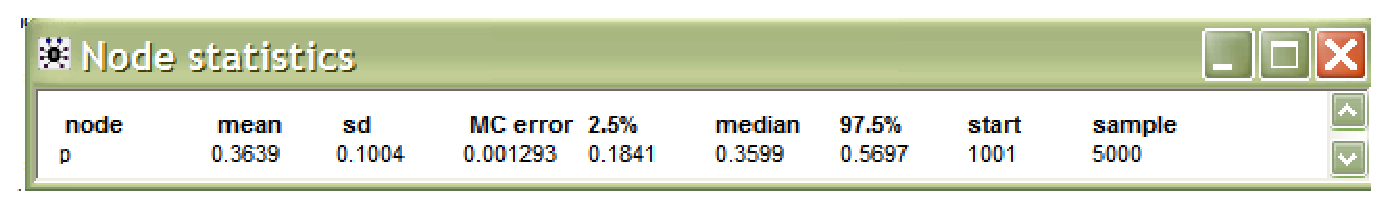
\includegraphics{binomial-results.eps}}
\end{center}
\caption{Results of a {\tt WinBUGS} analysis with the made up allele
  count data from {\it Desmodium cuspidatum}.}
\label{fig:binomial-results}
\end{figure}

The column headings in Figure~\ref{fig:binomial-results} should be
fairly self-explanatory, except for the one labeled {\tt MC
  error}.\footnote{If you're interested in what {\tt MC error} means,
  ask. Otherwise, I don't plan to say anything about it.} {\tt mean}
is the posterior mean. It's our best guess of the value for the
frequency of the {\it fast\/} allele. {\tt s.d.} is the posterior
standard deviation. It's our best guess of the uncertainty associated
with our estimate of the frequency of the {\it fast\/} allele. The
2.5\%, 50\%, and 97.5\% columns are the percentiles of the posterior
distribution. The [2.5\%, 97.5\%] interval is the 95\% credible
interval, which is analogous to the 95\% confidence interval in
classical statistics, except that we can say that there's a 95\%
chance that the frequency of the {\it fast\/} allele lies within this
interval.\footnote{If you don't understand why that's different from a
  standard confidence interval, ask me about it.} Since the results
are from a simulation, different runs will produce slightly different
results. In this case, we have a posterior mean of about 0.36 (as
opposed to the maximum-likelihood estimate of 0.35), and there is a
95\% chance that $p$ lies in the interval [0.18, 0.57].\footnote{See
  the Summer Institute notes for more details on why the Bayesian
  estimate of $p$ is different from the maximum-likelihood
  estimate. Suffice it to say that when you have a reasonable amount
  of data, the estimates are barely distinguishable.}

\section*{Returning to the ABO example}

Here's data from the ABO blood group:\footnote{This is almost the last
time! I promise.}
\begin{center}
\begin{tabular}{l|ccccc}
\hline\hline
Phenotype &   A &  AB &   B &   O & Total \\
Observed  & 862 & 131 & 365 & 702 & 2060 \\
\hline
\end{tabular}
\end{center}
To estimate the underlying allele frequencies, $p_A$, $p_B$, and
$p_O$, we have to remember how the allele frequencies map to phenotype
frequencies:\footnote{Assuming genotypes are in Hardy-Weinberg
  proportions. We'll relax that assumption later.}
\begin{eqnarray*}
\hbox{Freq}(A) &=& p_A^2 + 2p_Ap_O \\
\hbox{Freq}(AB) &=& 2p_Ap_B \\
\hbox{Freq}(B) &=& p_B^2 + 2p_Bp_O \\
\hbox{Freq}(O) &=& p_O^2 \quad .
\end{eqnarray*}
Hers's the {\tt WinBUGS} code we use to estimate the allele
frequencies:
\begin{verbatim}
model {
   # likelihood 
   pi[1] <- p.a*p.a + 2*p.a*p.o
   pi[2] <- 2*p.a*p.b
   pi[3] <- p.b*p.b + 2*p.b*p.o
   pi[4] <- p.o*p.o
   x[1:4] ~ dmulti(pi[],n)

   # priors
   a1 ~ dexp(1)
   b1 ~ dexp(1)
   o1 ~ dexp(1)
   p.a <- a1/(a1 + b1 + o1)
   p.b <- b1/(a1 + b1 + o1)
   p.o <- o1/(a1 + b1 + o1)

   n <- sum(x[])
}

list(x=c(862, 131, 365, 702))
\end{verbatim}
The {\tt dmulti()} is a multinomial probability, a simple
generalization of the binomial probability to samples when there are
more than two categories. The priors are some mumbo jumbo necessary to
produce the rough equivalent of uniform [0,1] priors with more than
two alleles.\footnote{It produces a Dirichlet(1,1,1), if you really
  want to know.} {\tt sum()} is a built-in function that saves me the
trouble of calculating the sample size and ensures that the n in {\tt
  dmulti()} is consistent with the individual sample components. The
{\tt x=c()} produces a vector of counts arranged in the same order as
the frequencies in {\tt pi[]}. The results are in Figure~\ref{fig:abo}.
Notice that the posterior means are very close to the
maximum-likelihood estimates, but that we also have 95\% credible
intervals so that we have an assessment of how reliable the Bayesian
estimates are. Getting them from a likelihood analysis is possible,
but it takes a fair amount of additional work.

\begin{figure}
\begin{center}
  \resizebox{\textwidth}{!}{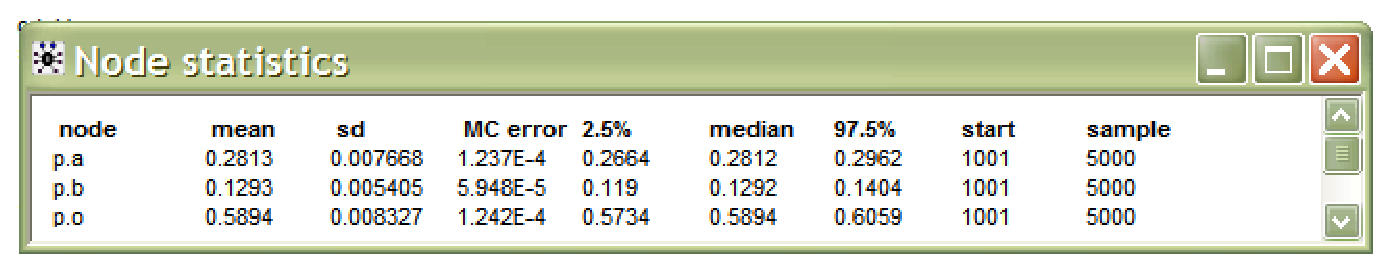
\includegraphics{multinomial-results.eps}}
\end{center}
\caption{Results of a {\tt WinBUGS} analysis of the ABO data.}
\label{fig:abo}
\end{figure}

\bibliography{popgen}
\bibliographystyle{plain}

\ccLicense

\end{document}
